\chapter{Real Estate: Control Before Ownership}

This chapter is based on the School of Hard Knocks interview with Matt Teifke, curated by LazyingArt LLC through Video2Book. There is no blackboard mathematics in this lecture and no retained screenshot evidence; the quantitative structure comes from the transcript itself. The central lesson is commercial: income changes when the unit of reward changes, ownership begins with control, and the visible headline number is only the beginning of the calculation.

\section{The Check That Reframed the Game}

The interview begins with the payoff before the background. Matt first remembers sitting with a local real estate broker when a \(\$200{,}000\) check arrives. The broker turns the check around and tells him that he will get there one day. Then the story jumps to the other end of the scale: Matt is working at Papa John's, delivering pizza and mopping the floor, when the first real estate call comes in.

That opening does an important piece of work. Before we know the degree path, the brokerage, the partner, or the later wholesale deal, we are shown a change in the unit of income. A wage job pays for time. A commission pays when a transaction closes. The commercial arithmetic begins there.

Let \(W\) denote the approximate paycheck scale Matt names from wage work, and let \(C_1\) denote the first real estate commission he reports. The transcript gives

\begin{equation}
W_{\text{pizza check}} \approx \$600,
\qquad
C_1 \approx \$6{,}000 \text{ to } \$7{,}000 .
\end{equation}

As a scale comparison, not an exact lifetime-income calculation,

\begin{equation}
\frac{\$6{,}000}{\$600}=10,
\qquad
\frac{\$7{,}000}{\$600}\approx 11.7 .
\end{equation}

So the first real money-making mechanism is not yet property ownership. It is exposure to a transaction system in which a single closing can be ten times the check Matt had been used to seeing. The force of dropping the mop is that the call belongs to a different economic rule.

\section{Learning Real Estate Until Ownership Became the Question}

After the preview, the host resets the interview and identifies Matt as the owner of Teifke Real Estate. The firm's ambition is also named at the beginning: Matt and his partners want to build an entrepreneurial real estate brokerage. That goal frames the biography that follows.

Matt's path is not described as a sudden leap. It is a repeated accumulation of real estate fluency. He was born in Cleveland, moved to Austin as a child, grew up with a single mother, and says his mother showed him what was possible through real estate. He got licensed at 17, went to Texas A\&M Corpus Christi, started at a mom-and-pop brokerage, and earned rookie of the year while still a full-time student.

The sequence then becomes more technical. He worked at a commercial brokerage in Round Rock, went to Texas A\&M for a financially based master's degree in real estate, worked at an apartment property, and got an appraisal license. The repeated question underneath the biography is the one Matt states directly: how do we learn enough about real estate to own it?

His first company with his wife was a third-party property-management company. Its scale is given as

\begin{equation}
D_{\text{managed}}=700\text{ doors}.
\end{equation}

That company was later sold. The next step was to team up with Alex Kaufman, a longtime childhood friend, and build the entrepreneurial brokerage that anchors the interview.

\subsection{Question \& Answer}

\paragraph{Question.}
Is college necessary for success in this path, or did it transfer into brokerage ownership and deal-making skill?

\paragraph{Answer.}
Matt's answer is deliberately not a clean yes. Necessary, no. Useful, yes, if one uses it. He says he now teaches a college class, and he tells students that a room of ten people interested in business contains a lifetime of possible mutual help. The missed opportunity is that many people simply attend class and leave.

The mechanism is therefore not a diploma by itself. It is a setting that can become a network, a skill base, and a repeated source of opportunity. In compact form,

\begin{equation}
\text{college value}
\neq
\text{degree alone},
\qquad
\text{college value}
\approx
\text{skills}+\text{network}+\text{initiative}.
\end{equation}

This is not a universal theorem about education. It is Matt's practical claim: college was not required, but it could be converted into relationships, financial understanding, and deal exposure.

\section{The First Deal and the Reversal of the Interview}

The host then takes Matt back to the first way he made money in real estate. Matt explains that he misunderstood the brokerage interview. He set up meetings, put on a suit and tie, and hoped that a broker would give him a job. Later he realized that, in many brokerages, the demand runs the other way as well: brokerages want agents because agents can produce transactions.

That reversal makes the earlier \(\$200{,}000\) check meaningful. It was not merely a motivational object. It showed the ceiling of a transaction world before Matt had entered it. He took the local broker's offer, canceled the other interviews, and began working at the brokerage while still keeping his pizza job because he needed money.

Then the first closing arrives. Matt says he took the call while mopping, closed the deal, and made about \(\$6{,}000\) or \(\$7{,}000\). He compares it with ordinary checks of about \(\$600\), and with earlier full-time checks of perhaps \(\$1{,}500\) or \(\$2{,}000\). The point is the same as in the opening, but now we understand the mechanism: the agent is paid from the closed transaction.

If \(C\) denotes a gross commission, the next question is who keeps what fraction of \(C\). That question leads directly into the transition from agent to broker.

\section{From Agent to Broker}

A licensed agent, as Matt explains it, cannot simply operate alone. Every agent must have a broker. The broker is the responsible party under whom agents work. So the move from agent to brokerage owner is not just a move from smaller income to larger income; it is a move from producing transactions to carrying responsibility for the structure that produces them.

\subsection{Question \& Answer}

\paragraph{Question.}
How does the transition from agent to broker work?

\paragraph{Answer.}
Matt describes the path as he experienced it. When he started, the requirement was two years and a certain amount of sales. Just before he reached that point, he says the rule changed to four years. He also describes a transaction point system, saying he believes the requirement was about 900 points, along with real estate classes, credit hours, and a licensing test. His college degree and master's degree satisfied the credit-hour side.

We should state these as transcript claims, not current legal guidance. In the notation of the chapter,

\begin{equation}
T_{\text{experience}}=4\text{ years},
\qquad
P_{\text{points}}\approx 900 .
\end{equation}

The important transition is from qualification to liability. Once licensed as the broker, Matt says, one becomes the person on the hook: responsible for training, support, and the agents' work.

\begin{table}
\centering
\begin{tabular}{|p{0.30\linewidth}|p{0.58\linewidth}|}
\hline
Stage & Function in Matt's description \\
\hline
Licensed agent & Works under a broker and earns through closed transactions. \\
\hline
Broker candidate & Accumulates experience time, transactions, points, classes, credit hours, and passes the test. \\
\hline
Broker & Becomes responsible for supervision, training, support, and the brokerage structure. \\
\hline
\end{tabular}
\caption{Transcript-grounded reconstruction of the agent-to-broker ladder.}
\end{table}

The economics arrive immediately after the licensing path. Matt says Teifke Real Estate uses a 90-10 split: the agent keeps 90 percent and the brokerage takes 10 percent. His first brokerage, by contrast, used a 50-50 split. If \(C\) is gross commission from a closed deal, then

\begin{align}
\text{Current split:}\qquad
C_{\text{agent}}&=0.90C,
&
C_{\text{brokerage}}&=0.10C,\\
\text{First brokerage:}\qquad
C_{\text{agent}}&=0.50C,
&
C_{\text{brokerage}}&=0.50C.
\end{align}

The equation is simple, but the business choice is not. A brokerage can take a larger share of each transaction, or it can give agents a larger share and try to win through volume, culture, training, support, and entrepreneurial energy.

\section{The Cost of Being on the Hook}

The host then asks what is hardest about owning a brokerage. Matt's answer moves us from formal licensing into operating reality. Deals fall apart. Lawsuits appear. Complaints arrive. The owner still has to show up and lead the team while carrying personal pressure.

This section is the other side of the brokerage split. The 10 percent is not free money. In Matt's description it is attached to responsibility. We can summarize the claim schematically:

\begin{equation}
C_{\text{brokerage}}
\quad \longleftrightarrow \quad
\text{training}+\text{support}+\text{risk bearing}+\text{leadership}.
\end{equation}

This is not an accounting identity. It is the operating logic Matt is describing. To own the brokerage is to own a position in the system, and that position includes pressure when the system misfires.

\section{Partnership as Operating Design}

The next movement is partnership. The host notes that Matt has a partner, Alex, and asks what qualities matter when choosing one. Matt begins with a hard claim: one in twenty partnerships work out, if that. Then he does not give a checklist. He tells the story of how trust became earned.

Alex was a childhood connection. Matt describes his addiction, jail, recovery, and the caution Matt felt when they first began working together. The trust was not assumed; it was tested in small assignments. Matt would tell Alex to knock 10 doors, and Alex would knock 100. He would ask him to call people, and Alex would call ten times the amount. Over two or three years, they owned four or five properties together.

\begin{align}
10\text{ doors assigned} &\longrightarrow 100\text{ doors knocked},\\
1\text{ unit of calling requested} &\longrightarrow 10\text{ units of calling performed},\\
2\text{ to }3\text{ years} &\longrightarrow 4\text{ to }5\text{ jointly owned properties}.
\end{align}

Only after that history does the partnership become a formal operating design. Alex is the operations person: counting the money, keeping the firm profitable, hiring, and firing if necessary. Matt's role is networking, building relationships, talking to people, and generating ideas. Using the language of Traction, Matt describes Alex as the implementer and himself as the visionary.

\begin{figure}
\centering
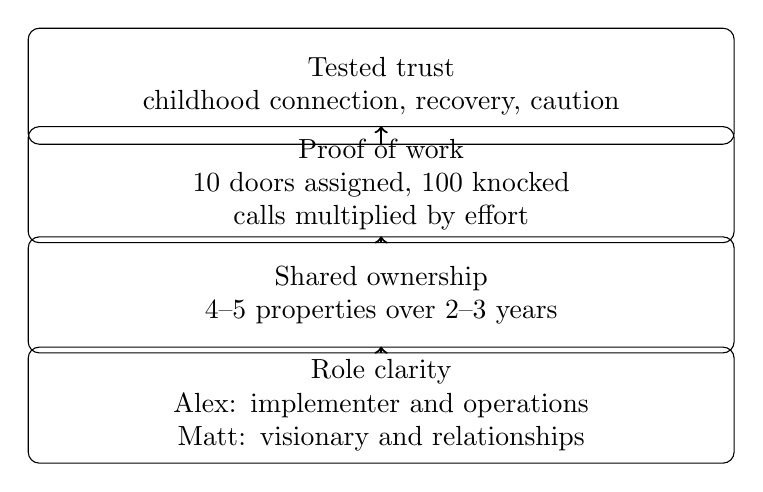
\begin{tikzpicture}[
  box/.style={draw, rounded corners, align=center, text width=0.72\linewidth, minimum height=0.58in},
  arrow/.style={->, thick}
]
\node[box] (trust) at (0,0) {Tested trust\\childhood connection, recovery, caution};
\node[box] (proof) at (0,-1.25) {Proof of work\\10 doors assigned, 100 knocked\\calls multiplied by effort};
\node[box] (assets) at (0,-2.65) {Shared ownership\\4--5 properties over 2--3 years};
\node[box] (roles) at (0,-4.05) {Role clarity\\Alex: implementer and operations\\Matt: visionary and relationships};
\draw[arrow] (trust) -- (proof);
\draw[arrow] (proof) -- (assets);
\draw[arrow] (assets) -- (roles);
\end{tikzpicture}
\caption{Transcript-grounded reconstruction of how trust becomes an operating partnership.}
\end{figure}

The general lesson is sharper than ``find a good partner.'' In this account, a partner becomes legible through repeated behavior under small tests. Then the business becomes scalable when the partners stop duplicating each other and divide the system into complementary functions.

\section{The Wholesale Deal}

The host asks about best and worst financial decisions and, within that, the biggest deal. Matt answers the biggest-deal part first: a \(\$700{,}000\) to \(\$780{,}000\) wholesale fee, made among three partners. The host pauses and asks him to explain wholesaling. That pause should remain, because this is the cleanest transaction mechanism in the interview.

\subsection{Question \& Answer}

\paragraph{Question.}
What is wholesaling in this example?

\paragraph{Answer.}
Matt's example is concrete. They put a property under contract. The seller did not want brokers, so they approached the transaction as investors. The contract price was about \(\$2{,}000{,}000\). They had a stated 3 percent commission going to themselves. They put up earnest money and option money of about \(\$20{,}000\). In Matt's phrase, they controlled the piece of paper, and that control gave them the economic opportunity.

Let

\begin{equation}
P_{\text{contract}}=\$2{,}000{,}000,
\qquad
E+O\approx \$20{,}000,
\qquad
A=9.5\text{ acres}.
\end{equation}

They then called builders, developers, and other possible buyers. The property was nine and a half acres in Round Rock, and Matt says they also wanted to buy it themselves because it was a commercial property. The outside offer came in at about

\begin{equation}
P_{\text{offer}}=\$2{,}700{,}000.
\end{equation}

A cautious reconstruction of the gross spread is therefore

\begin{align}
\Delta P
  &=P_{\text{offer}}-P_{\text{contract}}\\
  &=\$2{,}700{,}000-\$2{,}000{,}000\\
  &=\$700{,}000.
\end{align}

That arithmetic agrees with the later statement that they made the 700K, but the transcript also gives the wholesale fee as \(\$700{,}000\) to \(\$780{,}000\). We should preserve the range:

\begin{equation}
F_{\text{wholesale}}
\approx
\$700{,}000\text{ to }\$780{,}000.
\end{equation}

Matt also says they made the 3 percent commission. If we compute that on the stated \(\$2{,}000{,}000\) contract price, then

\begin{equation}
C_{\text{commission}}
=
0.03 \times \$2{,}000{,}000
=
\$60{,}000.
\end{equation}

That is a reconstruction for scale. The transcript gives the 3 percent figure but does not provide the full closing statement.

\begin{figure}
\centering
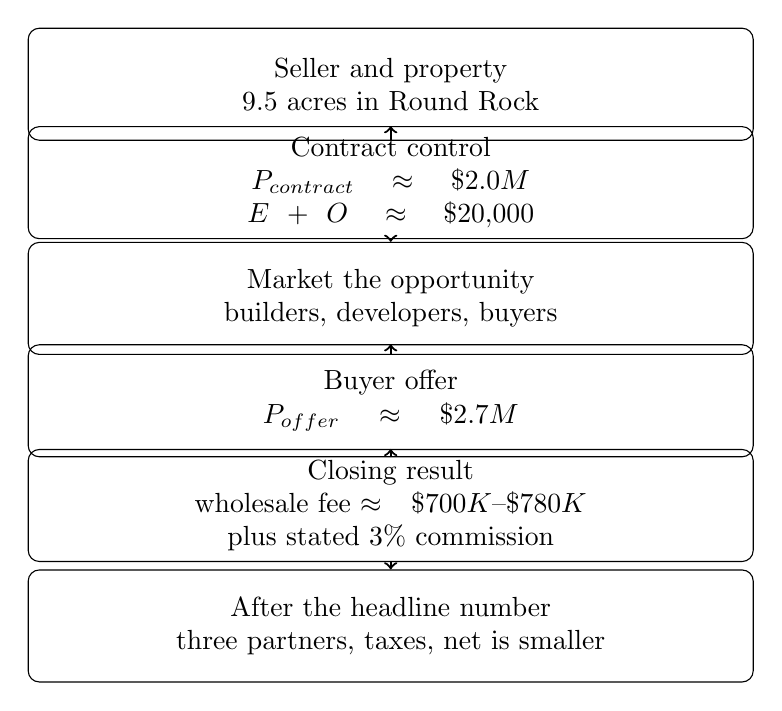
\begin{tikzpicture}[
  box/.style={draw, rounded corners, align=center, text width=0.74\linewidth, minimum height=0.56in},
  arrow/.style={->, thick}
]
\node[box] (seller) at (0,0) {Seller and property\\9.5 acres in Round Rock};
\node[box] (contract) at (0,-1.25) {Contract control\\\(P_{\text{contract}}\approx \$2.0\text{M}\)\\\(E+O\approx \$20{,}000\)};
\node[box] (market) at (0,-2.72) {Market the opportunity\\builders, developers, buyers};
\node[box] (offer) at (0,-4.02) {Buyer offer\\\(P_{\text{offer}}\approx \$2.7\text{M}\)};
\node[box] (close) at (0,-5.35) {Closing result\\wholesale fee \(\approx \$700\text{K}\)--\(\$780\text{K}\)\\plus stated 3\% commission};
\node[box] (after) at (0,-6.88) {After the headline number\\three partners, taxes, net is smaller};
\draw[arrow] (seller) -- (contract);
\draw[arrow] (contract) -- (market);
\draw[arrow] (market) -- (offer);
\draw[arrow] (offer) -- (close);
\draw[arrow] (close) -- (after);
\end{tikzpicture}
\caption{Transcript-grounded reconstruction of the wholesale-control sequence.}
\end{figure}

This is the most important quantitative example in the lecture because it separates ownership from control. The valuable object in the middle of the transaction was not yet the land itself. It was the contract position and the ability to transfer that position.

If the wholesale fee were split evenly among three partners, a rough pre-tax share would be

\begin{equation}
\frac{F_{\text{wholesale}}}{3}
\approx
\$233{,}333 \text{ to } \$260{,}000.
\end{equation}

That is not a final net proceeds calculation. Matt explicitly says they paid a huge tax and that the headline number was not nearly as much as it seemed. The right lesson is therefore not the glamour of the gross fee, but the mechanism: contract control, buyer demand, closing, split, and tax drag.

\section{Risk, Regret, and the Clear Goal}

After the wholesale explanation, the host circles back to best and worst financial decisions. Matt says they have perhaps 130 properties, but names the worst decision as cannabis stock. He says he is down multiple millions and describes daily mark-to-market movements of \(\$60{,}000\) to \(\$100{,}000\).

\begin{equation}
L_{\text{total}}=\text{multiple millions},
\qquad
\Delta L_{\text{daily}}\approx \$60{,}000\text{ to }\$100{,}000.
\end{equation}

He names Acreage and says he still believes in the industry and the company. He states that the company did \(\$67{,}000{,}000\) in revenue last quarter while being valued at \(\$40{,}000{,}000\). As testimony, the comparison is

\begin{equation}
R_{\text{quarter}}\approx \$67{,}000{,}000,
\qquad
V_{\text{company}}\approx \$40{,}000{,}000.
\end{equation}

The arithmetic ratio is

\begin{equation}
\frac{R_{\text{quarter}}}{V_{\text{company}}}
\approx
1.675.
\end{equation}

We should not turn that into investment advice. It is Matt's explanation of why he sees the position as early while also admitting the pain of the decline.

His best financial decision is not a stock or a property. It is partnering with Alex. That answer loops back to the earlier section: the strongest compounding asset in this account is not only a deal skill, but a trusted operating relationship attached to a clear goal.

The final part of the interview broadens the texture of the business. Matt tells a strange property-management story about his pregnant wife being chased at a managed property, and another about negotiating a deal at an RV park over a beer. These are not side jokes; they remind us that real estate is full of irregular human situations. The operator has to work inside that mess without being surprised by it every day.

When the host asks about the next ten years, Matt comes back to clarity. He says he is driven, shaped partly by his mother, and grateful to have a clear vision. He does not claim to be constantly inspired. He says the goal is clear, and that agents regularly tell the team the brokerage changed their lives. That feedback is what keeps the effort going.

\section{Summary}

The lecture unfolds as a sequence of increasingly concrete forms of control. First, Matt encounters commission income as a scale change from wage work: roughly \(\$600\) checks versus a first closing around \(\$6{,}000\) to \(\$7{,}000\). Then he accumulates fluency through licensing, college, brokerage work, appraisal, property management, and a 700-door company.

The middle of the interview explains how an agent becomes a broker as Matt experienced it: experience time, transactions, points, classes, credit hours, testing, and then responsibility. The 90-10 split is meaningful only when paired with being on the hook. Partnership then becomes operating design: tested trust, repeated overdelivery, shared ownership, and divided roles.

The wholesale deal gives the clearest arithmetic. A \(\$2{,}000{,}000\) contract position, about \(\$20{,}000\) of earnest and option money, outreach to buyers, and a \(\$2{,}700{,}000\) offer created a reported \(\$700{,}000\) to \(\$780{,}000\) wholesale fee, before partner splits and taxes. The closing lesson is not that wealth is clean or automatic. In this interview it is built through control, relationships, repeated effort, risk, tax consequences, and a goal clear enough to keep returning to.